% Template for Elsevier CRC journal article
% version 1.2 dated 09 May 2011

% This file (c) 2009-2011 Elsevier Ltd.  Modifications may be freely made,
% provided the edited file is saved under a different name

% This file contains modifications for Transportation Research Procedia

% Changes since version 1.1
% - added "procedia" option compliant with ecrc.sty version 1.2a
%   (makes the layout approximately the same as the Word CRC template)
% - added example for generating copyright line in abstract

%-----------------------------------------------------------------------------------

%% This template uses the elsarticle.cls document class and the extension package ecrc.sty
%% For full documentation on usage of elsarticle.cls, consult the documentation "elsdoc.pdf"
%% Further resources available at http://www.elsevier.com/latex

%-----------------------------------------------------------------------------------

%%%%%%%%%%%%%%%%%%%%%%%%%%%%%%%%%%%%%%%%%%%%%%%%%%%%%%%%%%%%%%
%%%%%%%%%%%%%%%%%%%%%%%%%%%%%%%%%%%%%%%%%%%%%%%%%%%%%%%%%%%%%%
%%                                                          %%
%% Important note on usage                                  %%
%% -----------------------                                  %%
%% This file should normally be compiled with PDFLaTeX      %%
%% Using standard LaTeX should work but may produce clashes %%
%%                                                          %%
%%%%%%%%%%%%%%%%%%%%%%%%%%%%%%%%%%%%%%%%%%%%%%%%%%%%%%%%%%%%%%
%%%%%%%%%%%%%%%%%%%%%%%%%%%%%%%%%%%%%%%%%%%%%%%%%%%%%%%%%%%%%%

%% The '3p' and 'times' class options of elsarticle are used for Elsevier CRC
%% The 'procedia' option causes ecrc to approximate to the Word template
\documentclass[3p,times,procedia]{elsarticle}
\flushbottom

%% The `ecrc' package must be called to make the CRC functionality available
\usepackage{ecrc}
%\usepackage{amsmath}


%% The ecrc package defines commands needed for running heads and logos.
%% For running heads, you can set the journal name, the volume, the starting page and the authors

%% set the volume if you know. Otherwise `00'
\volume{00}

%% set the starting page if not 1
\firstpage{1}

%% Give the name of the journal
\journalname{Transportation Research Procedia}

%% Give the author list to appear in the running head
%% Example \runauth{C.V. Radhakrishnan et al.}
\runauth{J. Raimbault}

%% The choice of journal logo is determined by the \jid and \jnltitlelogo commands.
%% A user-supplied logo with the name <\jid>logo.pdf will be inserted if present.
%% e.g. if \jid{yspmi} the system will look for a file yspmilogo.pdf
%% Otherwise the content of \jnltitlelogo will be set between horizontal lines as a default logo

%% Give the abbreviation of the Journal.
\jid{aaspro}

%% Give a short journal name for the dummy logo (if needed)
%\jnltitlelogo{Transportation Research Procedia}

%% Hereafter the template follows `elsarticle'.
%% For more details see the existing template files elsarticle-template-harv.tex and elsarticle-template-num.tex.

%% Elsevier CRC generally uses a numbered reference style
%% For this, the conventions of elsarticle-template-num.tex should be followed (included below)
%% If using BibTeX, use the style file elsarticle-num.bst

%% End of ecrc-specific commands
%%%%%%%%%%%%%%%%%%%%%%%%%%%%%%%%%%%%%%%%%%%%%%%%%%%%%%%%%%%%%%%%%%%%%%%%%%

%% The amssymb package provides various useful mathematical symbols

\usepackage{amssymb}
%% The amsthm package provides extended theorem environments
%% \usepackage{amsthm}

%% The lineno packages adds line numbers. Start line numbering with
%% \begin{linenumbers}, end it with \end{linenumbers}. Or switch it on
%% for the whole article with \linenumbers after \end{frontmatter}.
%% \usepackage{lineno}

%% natbib.sty is loaded by default. However, natbib options can be
%% provided with \biboptions{...} command. Following options are
%% valid:

%%   round  -  round parentheses are used (default)
%%   square -  square brackets are used   [option]
%%   curly  -  curly braces are used      {option}
%%   angle  -  angle brackets are used    <option>
%%   semicolon  -  multiple citations separated by semi-colon
%%   colon  - same as semicolon, an earlier confusion
%%   comma  -  separated by comma
%%   numbers-  selects numerical citations
%%   super  -  numerical citations as superscripts
%%   sort   -  sorts multiple citations according to order in ref. list
%%   sort&compress   -  like sort, but also compresses numerical citations
%%   compress - compresses without sorting
%%
\biboptions{authoryear}

% \biboptions{}

% if you have landscape tables
\usepackage[figuresright]{rotating}
%\usepackage{harvard}
% put your own definitions here:x
%   \newcommand{\cZ}{\cal{Z}}
%   \newtheorem{def}{Definition}[section]
%   ...

% add words to TeX's hyphenation exception list
%\hyphenation{author another created financial paper re-commend-ed Post-Script}


%%%%%%%%%%%%%%%%%%
%% User-defined packages

\usepackage{bbm}

\usepackage[utf8]{inputenc}
\usepackage[T1]{fontenc}

\usepackage[french]{babel}

%\renewcommand{\abstractname}{Résumé}


% declarations for front matter

\begin{document}

\begin{frontmatter}

%% Title, authors and addresses

%% use the tnoteref command within \title for footnotes;
%% use the tnotetext command for the associated footnote;
%% use the fnref command within \author or \address for footnotes;
%% use the fntext command for the associated footnote;
%% use the corref command within \author for corresponding author footnotes;
%% use the cortext command for the associated footnote;
%% use the ead command for the email address,
%% and the form \ead[url] for the home page:
%%
%% \title{Title\tnoteref{label1}}
%% \tnotetext[label1]{}
%% \author{Name\corref{cor1}\fnref{label2}}
%% \ead{email address}
%% \ead[url]{home page}
%% \fntext[label2]{}
%% \cortext[cor1]{}
%% \address{Address\fnref{label3}}
%% \fntext[label3]{}

\dochead{19th EURO Working Group on Transportation Meeting, EWGT2016, 5-7 September 2016, Istanbul, Turkey}
%% Use \dochead if there is an article header, e.g. \dochead{Short communication}
%% \dochead can also be used to include a conference title, if directed by the editors
%% e.g. \dochead{17th International Conference on Dynamical Processes in Excited States of Solids}

\title{Investigation Empirique de l'Existence de l'Equilibre Utilisateur Statique}

%% use optional labels to link authors explicitly to addresses:
%% \author[label1,label2]{<author name>}
%% \address[label1]{<address>}
%% \address[label2]{<address>}



%\author[a]{First Author} 
%\author[b]{Second Author}
\author[a,b]{Juste Raimbault\corref{cor1}}

\address[a]{UMR CNRS 8504 G{\'e}ographie-cit{\'e}s, 13 rue du Four, 75006 Paris, France}
\address[b]{UMR-T IFSTTAR 9403 LVMT, Cit{\'e} Descartes, 77455 Champs-sur-Marne, France}

\begin{abstract}
L'Equilibre Utilisateur Statique est un cadre puissant pour l'étude théorique du trafic. Malgré l'hypothèse restreignante de stationnarité des flots qui intuitivement limite son application aux systèmes de trafic réels, de nombreux modèles opérationnels qui l'implémentent sont toujours utilisés sans validation empirique de l'existence de l'équilibre. Nous étudions celle-ci sur un jeu de données de trafic couvrant trois mois sur la région parisienne. L'implémentation d'une application d'exploration interactive de données spatio-temporelles permet de formuler l'hypothèse d'une forte hétérogénéité spatiale et temporelle, guidant les études quantitatives. L'hypothèse de flots localement stationnaires est invalidée en première approximation par les résultats empiriques, comme le montrent une forte variabilité spatio-temporelle des plus courts chemins et des mesures topologiques du réseau comme la centralité de chemin. De plus, le comportement de l'index d'autocorrelation spatiale pour les motifs de congestion à différentes portées spatiales suggère une évolution chaotique à l'échelle locale, en particulier lors des heures de pointe. Nous discutons finalement les implications de ces résultats empiriques et proposons des possibles développements futurs basés sur l'estimation de la stabilité dynamique au sens de Lyapounov des flots de trafic.
\end{abstract}

\begin{keyword}
Equilibre Utilisateur Statique \sep Visualisation de Données Spatio-temporelles \sep Stationnarité Spatio-temporelle \sep Stabilité Dynamique

%% keywords here, in the form: keyword \sep keyword

%% PACS codes here, in the form: \PACS code \sep code

%% MSC codes here, in the form: \MSC code \sep code
%% or \MSC[2008] code \sep code (2000 is the default)

\end{keyword}
\cortext[cor1]{Auteur correspondant. Tel.: +33140464000.% ; fax: +0-000-000-0000.
}
\end{frontmatter}

%\correspondingauthor[*]{Corresponding author. Tel.: +0-000-000-0000 ; fax: +0-000-000-0000.}
\email{juste.raimbault@polytechnique.edu}

%%
%% Start line numbering here if you want
%%
% \linenumbers

%% main text

%\enlargethispage{-7mm}

%%%%%%%%%%%%%%%%%%%%%%%
\section{Introduction}
\label{introduction}


La modélisation du trafic a été largement étudiée depuis les travaux séminaux de Wardrop (\cite{wardrop1952road}) : les enjeux économiques et techniques justifient entre autre le besoin d'une compréhension fine des mécanismes régissant les flots de trafic à différentes échelles. Différentes approches aux objectifs différents coexistent aujourd'hui, parmi lesquels on trouve par exemple les modèles dynamiques de micro-simulation, généralement opposés aux techniques de basant sur l'équilibre. Tandis que la validité des modèles microscopiques a été étudiée de façon conséquente et leur application souvent questionnée, la littérature est relativement pauvre en études empiriques assurant l'hypothèse d'équilibre stationnaire du cadre de l'Equilibre Utilisateur Statique (EUS). De nombreux développements plus réalistes on été documentés dans la littérature, tels l'Equilibre Utilisateur Dynamique Stochastique (EUDS) (voir pour une description par example~\cite{han2003dynamic}). A un niveau intermédiaire entre les cadres statiques et stochastiques se trouve l'Equilibre Utilisateur Stochastique Restreint, pour lequel les choix d'itinéraire des utilisateurs sont contraints à un ensemble d'alternatives réalistes (\cite{rasmussen2015stochastic}). D'autres extensions prenant en compte le comportement de l'utilisateur via des modèles de choix ont été proposé plus récemment, comme~\cite{zhang2013dynamic} qui inclut à la fois l'influence de la tarification routière et de la congestion sur le choix avec un modèle Probit. La relaxation d'autres hypothèses restrictives comme la maximisation pure de l'utilité par l'utilisateur ont aussi été introduites, tels l'Equilibre Utilisateur Borné décrit par~\cite{mahmassani1987boundedly}. Dans ce cadre, l'utilisateur est satisfait si son utilité tombe dans un intervalle et l'équilibre est achevé lorsque chaque utilisateur est satisfait. Les dynamiques résultantes sont plus complexes comme révélé par l'existence d'équilibres multiples, et permet de rendre compte de faits stylisés spécifiques comme des évolutions irréversibles du réseau comme développé par~\cite{guo2011bounded}. D'autres modèles d'attribution de trafic inspirés d'autres domaines ont également été plus récemment proposés: dans~\cite{puzis2013augmented}, une définition étendue de la centralité de chemin qui combine linéairement le centralité des flots non-contraints avec une centralité pondérée par le temps de parcours permet d'obtenir une forte corrélation avec les flots de trafic effectifs, fournissant ainsi un modèle d'attribution de trafic. Cela fournit également des applications pratiques comme l'optimisation de la distribution spatiale des capteurs de trafic.


Malgré ces nombreux développements, de nombreuses études et applications concrètes se reposent toujours sur l'Equilibre Utilisateur Statique. La région parisienne utilise par exemple un modèle statique (MODUS) pour gérer et planifier le trafic. \cite{leurent2014user} introduit un modèle statique de flots qui inclut les recherches locales et le choix du parking : il est légitime de s'interroger, en particulier à de si faibles échelles, si la stationnarité de la distribution des flots est une réalité. Une example d'exploration empirique des hypothèses classiques est donné par~\cite{zhu2010people}, pour lequel les choix d'itinéraires révélés sont étudiés. Les conclusions questionnent le ``premier principe de Wardrop'' qui implique que les utilisateurs choisissent parmi un ensemble d'alternatives parfaitement connu. Dans le même esprit, nous étudions l'existence possible de l'équilibre en pratique. Plus précisément, l'EUS suppose une distribution stationnaire des flots sur l'ensemble du réseau. Cette hypothèse reste valable dans le cas d'une stationnarité locale, tant que l'échelle temporelle d'évolution des paramètres est considérablement plus grande que les échelles typiques de voyage. Le second cas qui est plus plausible et de plus compatible avec les cadres théoriques dynamiques est testé ici.

La suite de ce travail s'organise ainsi : la procédure de collection de données ainsi que le jeu de données sont décrits ; nous présentons ensuite une application interactive pour l'exploration du jeu de données, dans le but de fournir une intuitions sur les motifs présents ; puis nous donnons divers résultats d'analyses quantitatives allant dans le sens d'indices convergents pour une non-stationnarité des flots de trafic ; nous discutons finalement les implications de ces résultats et des développements possibles.




%%%%%%%%%%%%%%%%%%%%%
\section{Collecte des données}


%%%%%%%%%%%%%%%%%%%%%
\subsection{Construction du jeu de données}


Nous proposons de travailler sur l'étude de cas de la région métropolitaine de Paris. Un jeu de données ouvert a été construit, comprenant les liens autoroutiers dans la région, par collecte des données publiques en temps réel des temps de parcours (disponible sur www.sytadin.fr). Comme rappelé par~\cite{bouteiller2013open}, la disponibilité de jeux de données ouverts pour les transports est loin d'être la règle, et nous contribuons ainsi à une ouverture par la construction de notre jeu de données. La procédure de collecte de données consiste en les points suivants, executés toutes les deux minutes par un script \texttt{python} :
\begin{itemize}
\item récupération de la page web brute donnant les informations de trafic
\item parsing du code html afin de récupérer les identifiants des liens de trafic et les temps de parcours correspondants
\item insertion des liens dans une base \texttt{sqlite} avec le temps courant.
\end{itemize}


Le script automatisé de collection des données continue d'enrichir la base au fur et à mesure du temps, permettant des développements futurs de ce travail sur un jeu de données plus large, et une réutilisation potentielle pour des travaux scientifiques ou opérationnels. La dernière version du jeu de données au format sqlite est disponible en ligne sous une Licence \emph{Creative Commons}\footnote{à l'adresse \texttt{http://37.187.242.99/files/public/sytadin{\_}latest.sqlite3}}.



%%%%%%%%%%%%%%%%%%%%%
\subsection{Description des données}


Une granularité de deux minutes a été obtenue pour une période de trois mois (de février 2016 à avril 2016 inclus. La granularité spatiale est en moyenne de 10km, les temps de trajet étant fournis pour les liens majeurs. Le jeu de données contient 101 liens. La variable brute utilisée est le temps de trajet effectif, à partir duquel il est possible de construire la vitesse de trajet et la vitesse relative de trajet, définie comme le rapport entre temps de trajet optimal (temps de trajet sans congestion, pris comme le temps minimal sur l'ensemble des pas de temps) et le temps de trajet effectif. La congestion est construite par inversion d'un fonction BPR simple avec exposant 1, i.e. en prenant $c_i = 1 - \frac{t_{i,min}}{t_i}$ avec $t_i$ temps de trajet effectif dans le lien $i$ et $t_{i,min}$ temps de trajet minimal.





%%%%%%%%%%%%%%%%%%%%%%
\section{Méthodes and Résultats}


%%%%%%%%%%%%%%%%%%%%%%
\subsection{Visualisation des motifs spatio-temporels de congestion}


Notre approche étant entièrement empirique, une bonne connaissance des motifs existants pour les variables de traffic, en particulier de leur variations spatio-temporelles, est crucial pour guider toute analyse quantitative. En s'inspirant de la littérature étudiant la validation empirique de modèles, plus précisément les techniques de \emph{Modélisation orientée-motifs} introduites par~\cite{grimm2005pattern}, nous nous intéressons au motifs macroscopiques à des échelles temporelles et spatiales données : d'une manière équivalente aux faits stylisés qui sont dans cette approches extraits d'un système avant de tenter de le modéliser, nous devons explorer les données de manière interactive dans le temps et l'espace afin d'identifier des motifs pertinents et les échelles associées. Une application web interactive a ainsi été implémentée pour explorer les données, à l'aide des packages \texttt{R} \texttt{shiny} et \texttt{leaflet}\footnote{le code source de l'application et des analyses est disponible sur le dépôt ouvert du projet à\\
\texttt{https://github.com/JusteRaimbault/TransportationEquilibrium}}.
Cela permet une visualisation dynamique des motifs de congestion sur l'ensemble du réseau ou dans une zone particulière grace au zoom. L'application est accessible en ligne à l'adresse \texttt{http://shiny.parisgeo.cnrs.fr/transportation}. La Figure~\ref{fig:fig-1} présente une capture d'écran de l'interface. La conclusion majeure de l'exploration interactive des données est qu'une grande hétérogénéité spatiale et temporelle est la règle. Le motif temporel le plus récurrent, la périodicité journalière des heures de pointe, est perturbée pour une proportion non négligeable de jours. En première approximation, les heures creuses peuvent être approchées par une distribution localement stationnaire des flots, tandis que les heures de pointe sont trop courtes pour pouvoir impliquer la validation de l'hypothèse d'équilibre. Concernant l'espace, aucun motif spatial particulier n'émerge clairement. Cela signifie que dans le cas d'une validité de l'équilibre utilisateur statique, les méta-paramètres régissant son établissement doivent varier à des échelles temporelles plus courtes qu'un jour. Nous postulons au contraire que le système de traffic est loin de l'équilibre, en particulier pendant les heures de pointe pendant lesquelles des transitions de phase critiques à l'origine des embouteillages émergent.

 

%%%%%%%%%%%%%%%%%%
\begin{figure}
\vspace{1cm}
\centering

\includegraphics[width=\textwidth]{gr1}
\caption{Capture de l'application web permettant l'exploration spatio-temporelle des données de traffic pour la région Parisienne. Il est possible de choisir date et heure (précision de 15min sur un mois, réduite par rapport au jeu de données initial pour des raisons de performance). Un graphe résume les motifs de congestion pour la journée courante.}
\label{fig:fig-1}
\end{figure}
%%%%%%%%%%%%%%%%%%



%%%%%%%%%%%%%%%%%%%%%%%%
\subsection{Variabilité Spatio-temporelle des Trajets}


A la suite de l'exploration interactive des données, nous proposons de quantifier la variabilité spatiale des motifs de congestion pour valider ou invalider l'intuition que si l'équilibre existe par rapport au temps, il est fortement dépendant de l'espace et localisé. La variabilité spatio-temporelle des plus courts chemins de trajet est une première façon d'étudier la stationnarité des flots d'un point de vue de théorie des jeux. En effet, l'Equilibre Utilisateur Statique est la distribution stationnaire des flots sous laquelle aucun utilisateur ne peut augmenter son temps de trajet en changeant son itinéraire. Une forte variabilité spatiale des plus courts chemins sur de courtes échelles spatiales révèle ainsi une non-stationnarité, puisque un même utilisateur prendra un chemin complètement différent après un court laps de temps et ne contribuera plus au même flot que précédemment. Une telle variabilité est en effet observée sur un nombre non-négligeable de chemins pour chaque jour du jeu de données. La figure~\ref{fig:fig-2} montre un exemple de variation spatiale extrême d'un trajet pour une paire Origine-Destination particulière.

L'exploration systématique de la variabilité du temps de trajet sur l'ensemble du jeu de données, et des distances de trajet associées, confirme, comme présenté en figure~\label{fig:fig-3}, que la variation absolue du temps de trajet présente fréquemment une forte variation de son maximum sur l'ensemble des paires O-D, jusqu'à 25 minutes avec une moyenne temporelle locale autour de 10 minutes. La variabilité spatiale correspondante entraine des détours allant jusqu'à 35km.




%%%%%%%%%%%%%%%%%%%
\begin{figure}
\centering
\vspace{1.5cm}
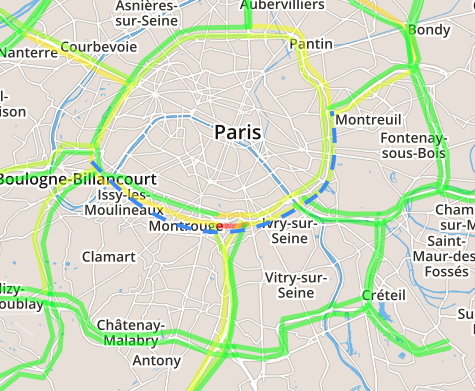
\includegraphics[width=0.47\textwidth]{gr21}\hfill
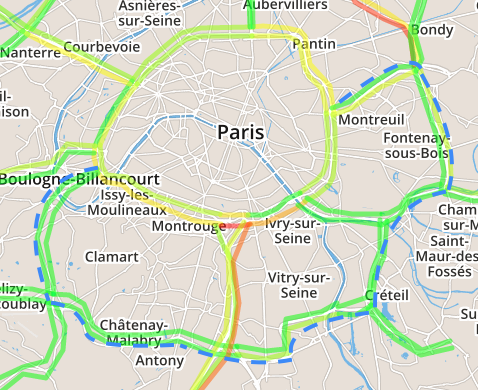
\includegraphics[width=0.47\textwidth]{gr22}
\caption{Variabilité spatiale d'un plus court chemin en temps de trajet (trajet du plus court chemin en pointillé bleu). Dans un intervalle de seulement 10 minutes, entre le 11/02/2016 00:06 (à gauche) et le 11/02/2016 00:16 (à droite), le plus court chemin entre Porte d'Auteuil à l'ouest et Porte de Bagnolet à l'est, augmente en distance effective de $\simeq 37$km (avec une augmentation du temps de trajet de seulement 6 minutes), à cause d'une forte perturbation sur le périphérique parisien.} 
\label{fig:fig-2}
\end{figure}
%%%%%%%%%%%%%%%%%%%



%%%%%%%%%%%%%%%%%%%
\begin{figure}[t]\vspace*{4pt}
\centering
\centerline{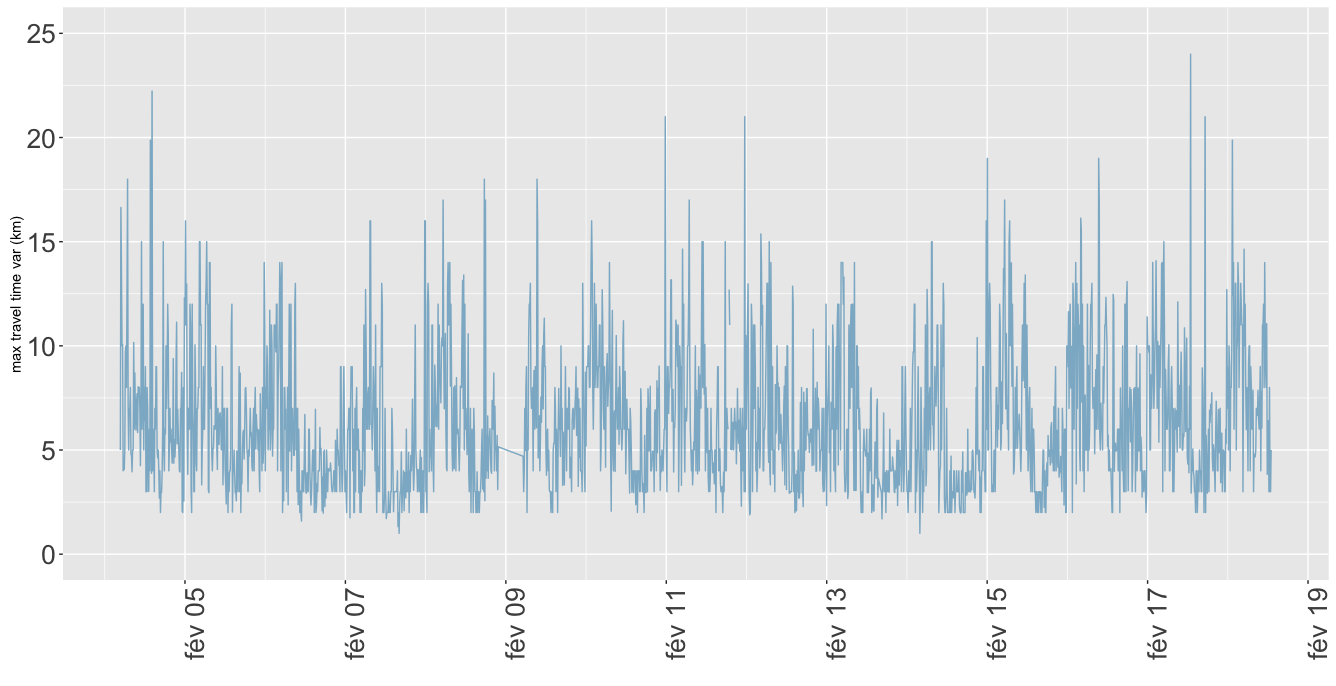
\includegraphics[width=0.8\textwidth]{gr31}}
\centerline{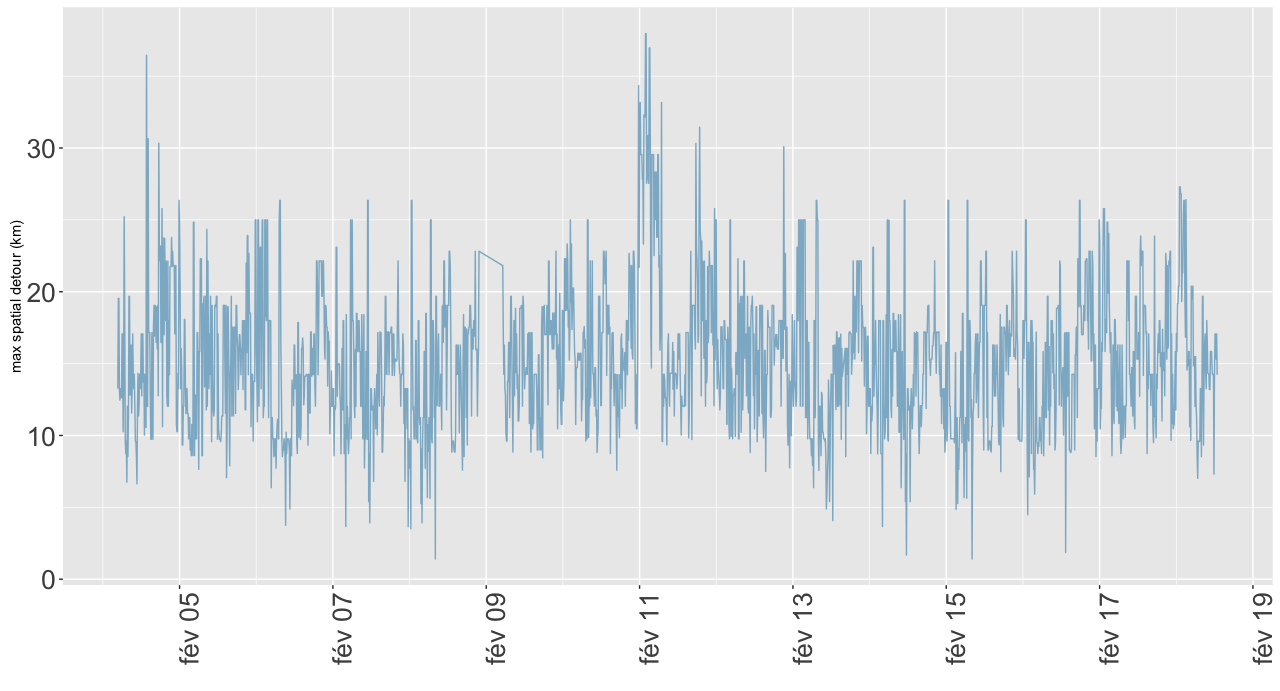
\includegraphics[width=0.8\textwidth]{gr32}}
\caption{Variabilité maximale du temps de trajet (en haut) en minutes et de la distance de trajet correspondante (en bas) pour un échantillon de deux semaines. Le graphe représente le maximum sur l'ensemble des paires Origine-Destination de la variabilité absolue entre deux pas de temps consécutifs. Les heures de pointe induisent une forte variabilité du temps de trajet, allant jusqu'à 25 minutes et une variabilité de distance jusqu'à 35km.}
\label{fig:fig-3}
\end{figure}
%%%%%%%%%%%%%%%%%%%




%%%%%%%%%%%%%%%%%%%
\subsection{Stabilité des mesures de réseau}


La variabilité des trajectoires potentielles observée dans la section précédente peu être confirmée par l'étude de la variabilité des propriétés du réseau. En particulier, les mesures topologiques de réseau capturent les motifs globaux dans un réseau de transport. Les mesures de centralité et de connectivité des noeuds sont des indicateurs classiques pour la description des réseaux de transport comme rappelé par~\cite{bavoux2005geographie}. La littérature en transports a développé des mesures de réseau élaborées et opérationnelles, comme des mesures de robustesse pour identifier les liens critiques et mesurer la résilience globale du réseau aux perturbations (un exemple parmi d'autres est l'indice de \emph{Robustesse du Réseau Effective} introduit dans ~\cite{sullivan2010identifying}).


Plus précisément, nous étudions la centralité de chemin du réseau de transport, défini pour un noeud comme le nombre de plus courts chemins passant par celui-ci, i.e. par l'équation

%%%%%%%%%%%%%%%
% equation betweeness
\begin{equation}
b_i = \frac{1}{N(N-1)}\cdot \sum_{o\neq d \in V}\mathbbm{1}_{i\in p(o\rightarrow d)}
\end{equation}
%%%%%%%%%%%%%%%

où $V$ est l'ensemble des sommets du réseau de taille $N$, et $p(o\rightarrow d)$ est l'ensemble des noeuds sur le plus court chemin entre les sommets $o$ et $d$ (le plus court chemin étant calculé avec le temps de trajet effectif). Cette mesure de centralité est plus adaptée que d'autre dans notre cas, comme la centralité de proximité qui n'inclut pas la congestion potentielle comme la centralité de chemin.


Nous montrons en Figure 4 la variation relative absolue du maximum de la centralité de chemin, pour la même fenêtre temporelle que les indicateurs empiriques précédents. Plus précisément, elle est définie par


%%%%%%%%%%%%%%%
% eq relative variability
\begin{equation}
\Delta b(t) = \frac{\left|\max_i (b_i(t + \Delta t)) - \max_i (b_i(t))\right|}{\max_i (b_i(t))}
\end{equation}
%%%%%%%%%%%%%%%


où $\Delta t$ est le pas de temps du jeu de données (la plus petite fenêtre temporelle sur laquelle une variabilité peut être capturée). Cette variation relative absolue a une signification directe : une variation de 20\% (qui est atteinte un nombre significatif de fois comme montré en Figure~\ref{fig:fig-4}) implique dans le cas d'une variation négative, qu'au moins cette proportion de trajectoires potentielles ont changé et que la potentielle congestion locale a décru de la même proportion. Dans le cas d'une variation positive, un seul noeud a capturé au moins 20\% des trajets. Sous l'hypothèse (qu'on ne tente pas de vérifier ici et qu'on peut également supposer non vérifiée comme montré par~\cite{zhu2010people}, mais que l'on utilise comme un outil pour donnée une intuition sur la signification concrète de la variabilité de la centralité) que les utilisateurs choisissent rationnellement le plus court chemin, et supposant que la majorité des trajets est réalisées, une telle variation de la centralité implique une variation similaire dans les flots effectifs, conduisant à la conclusion qu'ils ne peuvent être stationnaires ni dans le temps (au moins sur une échelle plus grande que $\Delta t$) ni dans l'espace.




%%%%%%%%%%%%%%%%%%%
\begin{figure}
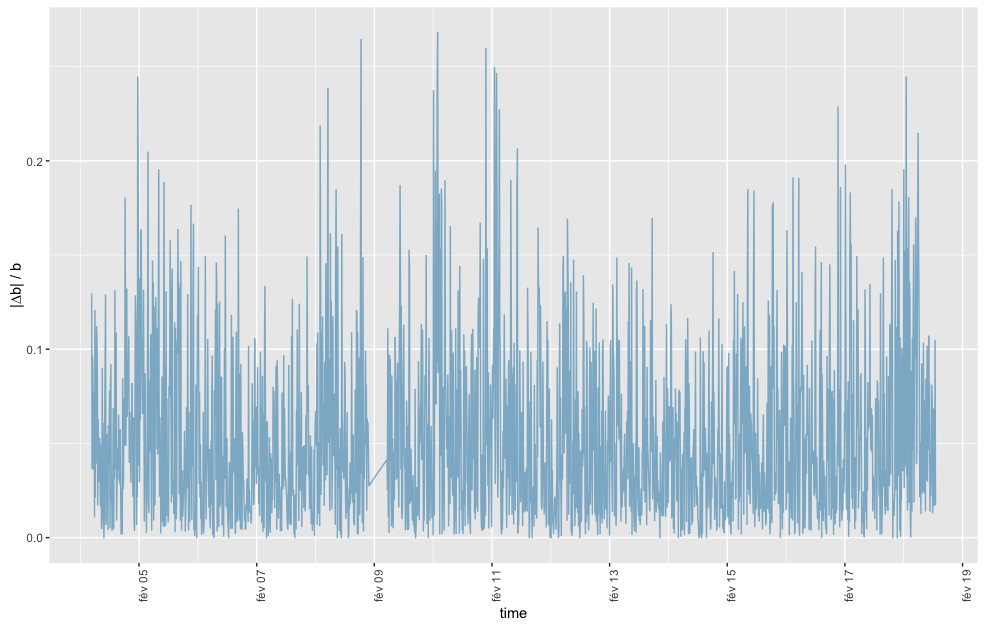
\includegraphics[width=\textwidth]{gr4}
\caption{Stabilité temporelle du maximum de la centralité de chemin. Le graphe montre dans le temps la dérivée normalisée du maximum de la centralité de chemin, qui capture ses variations relatives à chaque pas de temps. La valeur maximale de 25\% correspond à de très fortes perturbations du réseau sur les liens correspondants, puisque cela implique qu'au moins cette proportion d'utilisateurs prenant le lien dans des conditions précédentes doivent prendre un trajet complètement différent.}
\label{fig:fig-4}
\end{figure}
%%%%%%%%%%%%%%%%%%%





%%%%%%%%%%%%%%%%%%%
\subsection{Hétérogénéité spatiale de l'équilibre}


Afin d'obtenir un point de vue différent sur la variabilité spatiale des motifs de congestion, nous proposons d'utiliser un indice d'auto-corrélation spatiale, l'indice de Moran (défini par exemple dans~\cite{tsai2005quantifying}). Utilisé plus généralement en analyse spatiale, avec diverses applications allant de l'étude de la forme urbaine à la quantification de la ségrégation, il peut être appliqué à toute variable spatiale. Il permet d'établir des relations de voisinage et révèle la consistence spatiale locale d'un équilibre s'il est appliqué à une variable de traffic localisée. A un point donnée de l'espace, l'auto-corrélation locale pour la variable $c$ est calculée par

%%%%%%%%%%%%
% Moran index def
\begin{equation}
\rho_i = \frac{1}{K}\cdot \sum_{i\neq j}{w_{ij}\cdot (c_i - \bar{c})(c_j - \bar{c})}
\end{equation}
%%%%%%%%%%%%

où $K$ est une constante de normalisation égale à la somme des poids spatiaux fois la variance de la variable et $\bar{c}$ est la moyenne de la variable. Dans notre cas, nous choisissons des poids spatiaux de la forme $w_{ij} = \exp{\left(\frac{-d_{ij}}{d_0}\right)}$ avec $d_0$ distance typique de décroissance. L'auto-corrélation est calculée sur la congestion des liens, localisée au centre du lien. Elle capture ainsi les corrélations spatiales dans un rayon du même ordre que la distance de décroissance autour du point $i$. La moyenne sur l'ensemble des points fournit l'indice d'auto-corrélation spatiale $I$. Une stationnarité des flots devrait impliquer une stabilité temporelle de l'index. 

% rq : spatio-temporal stationarity has not been defined rigorously : could mean different things ? -> clarify that when integrate in thesis


La figure~\ref{fig:fig-5} présente l'évolution temporelle de l'auto-corrélation spatiale pour la congestion. Comme attendu, on observe une forte décroissance de l'auto-corrélation avec la distance de décroissance, à la fois sur l'amplitude et les moyennes temporelles. La forte variabilité temporelle implique de courtes échelles temporelles pour des fenêtres potentielles de stationnarité. Pour une distance de décroissance de 1km, en comparant l'auto-corrélation à la congestion (ajustée à l'échelle du graphe pour lisibilité), on observe que les fortes corrélations coincident avec les heures creuses, tandis que les heures de pointe correspondent à une décroissance des corrélations. Notre interprétation, combinée avec la variabilité observée des motifs spatiaux, est que les heures de pointe correspondent à un comportement chaotique du système, puisque les bouchons peuvent émerger dans n'importe quel lien du réseau : la corrélation disparait alors puisque l'espace des phases atteignables pour un système dynamique chaotique est rempli uniformément par les trajectoires, de façon équivalente à des vitesses relatives qui apparaitraient comme aléatoires et indépendantes.


%%%%%%%%%%%%%%%%
\begin{figure}
% Spatial 
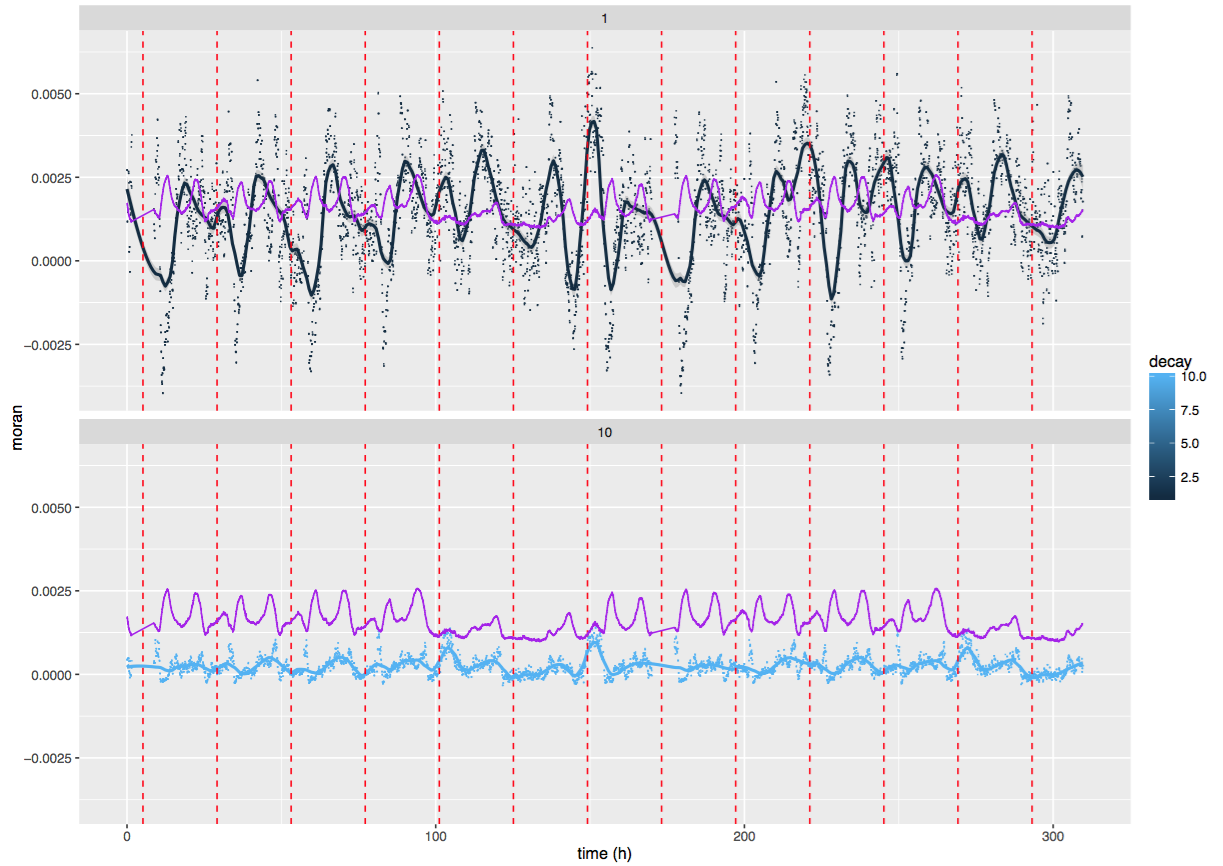
\includegraphics[width=\textwidth,height=0.6\textheight]{gr5}
\caption{Auto-corrélations spatiales pour les vitesses relatives sur deux semaines. Le graphe montre les valeurs de l'auto-corrélation dans le temps, pour des valeurs variables (1,10km) de la distance de décroissance. les valeurs intermédiaires de la distance de décroissance donnent une déformation relativement continue entre ces deux extrêmes. Les points sont lissés sur une fenêtre temporelle de 2h pour faciliter la lecture. Les lignes pointillées verticales correspondent à minuit de chaque jour. La courbe violette donne la vitesse relative, ajustée à l'échelle pour établir la correspondance entre les heures de pointe et les variations de l'auto-corrélation.}
\label{fig:fig-5}
\end{figure}
%%%%%%%%%%%%%%%%




%%%%%%%%%%%%%%%%%%%%
\section{Discussion}

\subsection{Implications théoriques et pratiques des conclusions empiriques}


Nous prétendons que les implications théoriques de ces résultats empiriques n'impliquent pas nécessairement un rejet total du cadre de l'Equilibre Utilisateur Statique, mais révèlent plutôt un besoin de plus fortes connexions entre la littérature théorique et les études empiriques. Si chaque nouveau cadre théorique introduit est généralement testé sur un cas ou plus, il n'existe pas de comparaisons systématiques de chacun sur des jeux de données de grande taille et variés, et pour des objectifs d'application différents (prédiction du traffic, reproduction de faits stylisés, etc.), à l'image des revues systématiques qui sont la règle en évaluation thérapeutique par exemple. Cela implique cependant des pratiques de partage des données et des modèles plus larges que celles existant couramment. La connaissance précise des potentialités d'application d'un cadre donné peut induire des développements inattendus comme l'intégration dans des modèles plus larges. L'exemple des études des interaction entre Transport et Usage du Sol (modèles \emph{LUTI}) est une bonne illustration d'un cas ou le EUS peut toujours être utilisé avec des motivations plus larges que la modélisation du traffic. \cite{kryvobokov2013comparison} décrit deux modèles \emph{LUTI}, dont l'un inclut deux équilibres pour les modèles de transport à quatre temps et pour l'évolution de l'usage du sol (localisation des ménages et emplois), l'autre étant dynamique. La conclusion est que chaque modèle à ses avantages au regard de l'objectif poursuivi, et que le modèle statique peut être utilisé pour comparer des politiques sur le temps long, tandis que le modèle dynamique fournit de l'information plus précise à de plus petites échelles temporelles. Dans le premier cas, un module de transport plus compliqué aurait été plus difficile à inclure, ce qui est un avantage du EUS dans ce cas.


Concernant les applications pratiques, il semble naturel que les modèles statiques ne devraient pas être utilisés pour la prédiction et la gestion du traffic sur de petites échelles temporelles (semaine ou jour) et que des efforts doivent être faits pour implémenter des modèles plus réalistes. Cependant, l'utilisation des modèles par la communautés des ingénieurs et des planificateurs n'est pas directement reliée aux enjeux académiques et à l'état de l'art dans le domaine. Dans le cas particulier de la France et des modèles de mobilité, \cite{commenges2013invention} a montré que les ingénieurs allaient jusqu'au point de construire des problèmes inexistants et d'implémenter les modèles correspondants qu'ils avaient importé d'un contexte géographique totalement différent (la planification aux Etats-Unis). L'utilisation d'un cadre ou d'un type de modèle a des raisons historiques qui peuvent être difficiles à surmonter.




\subsection{Vers des interprétations explicatives de la non-stationarité}


Une hypothèse qu'on peut formuler concernant l'origine de la non-stationnarité des flots dans le réseau, au regard de l'exploration des données et des analyses quantitatives, est que le réseau est au moins la moitié du temps fortement congestionné et dans un état critique. Les heures creuses sont les plus grandes fenêtres temporelles potentielles de stationnarité spatiale et temporelle, mais couvre moins de la moitié du temps. Comme déjà interprété dans le comportement de l'indicateur d'auto-corrélation, un comportement chaotique pourrait être à l'origine d'une telle variabilité lors des heures congestionnées. A la manière d'un fluide supercritique qui condense sous une perturbation externe infinitésimale, l'état d'un lien peut qualitativement changer par un petit incident, produisant une perturbation du réseau qui se propage et peut même s'amplifier. L'effet direct des évènements du traffic (incidents signalés ou accidents) ne peut pas être étudié sans source de données extérieure, et un enrichissement de la base de données dans cette direction pourrait être intéressante. Cela permettrait d'établir la proportion de perturbations qui paraissent avoir un effet direct et quantifier un niveau de caractère critique de la congestion du réseau dans le temps, ou d'étudier plus précisément des phénomènes localisés comme les conséquences d'un incident de traffic sur la voie opposée.


\subsection{Développements possibles}


Le travail futur pourra être planifié dans la direction d'une étude raffinée de la stabilité temporelle sur des zones du réseau, i.e. l'étude quantitative précise de la non-stationnarité des heures de pointes découverte ci-dessus. Pour cela nous proposons de calculer numériquement la stabilité de Liapounov du système dynamique régissant les flots de traffic, par l'intermédiaire d'algorithmes numériques comme ceux décrits par~\cite{goldhirsch1987stability}. La valeur des exposants de Liapounov fournit l'échelle de temps sur laquelle le système instable s'éloigne de l'équilibre. Leur comparaison avec la durée des heures de pointe et le temps de trajet moyen, sur différentes zones spatiales et différentes échelles, devrait fournir plus d'information sur une possible validité de l'hypothèse de stationnarité locale. Cette technique a déjà été introduite à une autre échelle dans les études de transport, comme e.g.~\cite{tordeux2016jam} qui étudie la stabilité des modèles de régulation de vitesse à l'échelle microscopique pour éviter l'émergence de congestion.


D'autres directions de recherche peuvent consister en le test des autres hypothèses du EUS (comme le choix rationnel du plus court chemin, qui serait cependant difficile à tester à un tel niveau d'agrégation, impliquant l'utilisation de modèles de simulation calibrés et cross-validés sur le jeu de données pour comparer différentes hypothèses, sans toutefois nécessairement une validation ou invalidation directe de l'hypothèse), ou le calcul empirique des paramètres dans les cadres d'Equilibre Utilisateur Stochastique ou Dynamique.



\section{Conclusion}

Nous avons décrit une étude empirique ayant pour but une étude simple, mais selon notre point de vue nécéssaire, de l'existence de l'équilibre utilisateur statique, plus précisément de sa stationnarité dans le temps et l'espace pour un réseau routier métropolitain principal. Un jeu de données de congestion du trafic est construite par collection de données, pour le réseau du Grand Paris sur 3 mois avec une granularité temporelle de 2 minutes. L'exploration interactive du jeu de données via une application web permettant la visualisation spatio-temporelle aide à guider les analyses quantitatives. La variabilité spatio-temporelle des plus courts chemins et de la topologie du réseau, en particulier la centralité de chemin, révèle que l'hypothèse de stationnarité ne tient généralement pas, ce qui est confirmé par l'étude de l'auto-corrélation spatiale de la congestion du réseau. Nous suggérons que nos résultats soulignent un besoin général de plus grandes connexions entre les études théoriques et empiriques, puisque cette étude permet de chasser les incompréhensions théoriques sur l'Equilibre Utilisateur Statique, et guider le choix d'application potentielles.






%% References
%%
%% Following citation commands can be used in the body text:
%% Usage of \cite is as follows:
%%   \cite{key}         ==>>  [#]
%%   \cite[chap. 2]{key} ==>> [#, chap. 2]
%%

%The citation must be used in following style: \cite{article-minimal} \cite{article-full} \cite{article-crossref} \cite{whole-journal}.
%% References with BibTeX database:

\bibliography{biblio}
\bibliographystyle{elsarticle-harv}





%%%%%%%%%%%%%%%%%%%%
% Original templates







%Here introduce the paper, and put a nome¬nclature if necessary, in a box with the same font size as the rest of the paper. The paragraphs continue from here and are only separated by headings, subheadings, images and formulae. The section headings are arranged by numbers, bold and 10 pt. Here follows further instructions for authors.

%\begin{nomenclature}
%\begin{deflist}[A]
%\defitem{A}\defterm{radius of}
%\defitem{B}\defterm{position of}
%\defitem{C}\defterm{further nomenclature continues down the page inside the text box\vspace*{-8pt}}
%\end{deflist}
%\end{nomenclature}
%\vspace*{0pt}

%\subsection{ Structure}
%Files must be in LaTeX format only and should be formatted for direct printing, using the CRC LaTeX template provided. Figures and tables should be embedded and not supplied separately. 

%Please make sure that you use as much as possible normal fonts in your documents. Special fonts, such as fonts used in the Far East (Japanese, Chinese, Korean, etc.) may cause problems during processing. To avoid unnecessary errors you are strongly advised to use the `spellchecker' function of TeX Editor. Follow this order when typing manuscripts: Title, Authors, Affiliations, Abstract, Keywords, Main text (including figures and tables), Acknowledgements, References, Appendix. Collate acknowledgements in a separate section at the end of the article and do not include them on the title page, as a footnote to the title or otherwise.

%Bulleted lists may be included and should look like this:
%\begin{itemize}[]
%\item First point
%\item Second point
%\item And so on
%\end{itemize}

%Ensure that you return to the `Els-body-text' style, the style that you will mainly be using for large blocks of text, when you have completed your bulleted list. 

%Please do not alter the formatting and style layouts which have been set up in this template document. As indicated in the template, papers should be prepared in single column format suitable for direct printing onto paper with trim size $192 \times 262$ mm. Do not number pages on the front, as page numbers will be added separately for the preprints and the Proceedings. Leave a line clear between paragraphs. All the required style templates are provided in the file ``LaTeX Template'' with the appropriate name supplied, e.g. choose 1. Els1st-order-head for your first order heading text, els-abstract-text for the abstract text etc.

%\subsection{ Tables}

%All tables should be numbered with Arabic numerals. Every table should have a caption. Headings should be placed above tables, left justified. Only horizontal lines should be used within a table, to distinguish the column headings from the body of the table, and immediately above and below the table. Tables must be embedded into the text and not supplied separately. Below is an example which the authors may find useful.

%\begin{table}[h]
%\caption{An example of a table.}
%\begin{tabular*}{\hsize}{@{\extracolsep{\fill}}lll@{}}
%\toprule
%An example of a column heading & Column A ({\it{t}}) & Column B ({\it{t}})\\
%\colrule
%And an entry &   1 &  2\\
%And another entry  & 3 &  4\\
%And another entry &  5 &  6\\
%\botrule
%\end{tabular*}
%\end{table}










%%\enlargethispage{12pt}

%\subsection{ Construction of references}

%References must be listed at the end of the paper. Do not begin them on a new page unless this is absolutely necessary. Authors should ensure that every reference in the text appears in the list of references and vice versa. Indicate references by \cite{clark} or \cite{Deal} or \cite{Fachinger2006} in the text. 

%Some examples of how your references should be listed are given at the end of this template in the `References' section, which will allow you to assemble your reference list according to the correct format and font size.

%Reference generation by using bibliography style commands for LaTeX template only.

%The author may use ``elsarticle-harv.bst'' as per the style required in document. The sample bib file could be referred. 
%If the author may using bibstyle for providing references author must comment the bibliography section in TeX file, Bibtex will generate the reference automatically.

%If the author may not able to view the references in output same could be done by copying the bibliography section from ``filename.bbl'' file and paste in TeX file.







%\subsection{Section headings}
%Section headings should be left justified, bold, with the first letter capitalized and numbered consecutively, starting with the Introduction. Sub-section headings should be in capital and lower-case italic letters, numbered 1.1, 1.2, etc,~and left justified, with second~and subsequent lines indented. All headings should have a minimum of two text lines after them before a page or column break.
%Ensure the text area is not blank except for the last page.

%\subsection{General guidelines for the preparation of your text}
%Avoid hyphenation at the end of a line. Symbols denoting vectors and matrices should be indicated in bold type. Scalar variable names should normally be expressed using italics. Weights and measures should be expressed in SI units. All non-standard abbreviations or symbols must be defined when first mentioned, or a glossary provided.

%\subsection{File naming and delivery}
%Please title your files in this order `procedia acronym\_conference acronym\_authorslastname'.  Submit both the source file and the PDF to the Guest Editor.

%Artwork filenames should comply with the syntax ``aabbbbbb.ccc'', where:\vspace*{-12pt}
%\begin{itemize}
%\item a = artwork component type
%\item b = manuscript reference code
%\item c = standard file extension

%Component types:
%\item gr = figure
%\item pl = plate
%\item sc = scheme
%\item fx = fixed graphic
%\end{itemize}


%\subsection{Footnotes}
%Footnotes should be avoided if possible. Necessary footnotes should be denoted in the text by consecutive superscript letters\footnote{Footnote text.}. The footnotes should be typed single spaced, and in smaller type size (8 pt), at the foot of the page in which they are mentioned, and separated from the main text by a one line space extending at the foot of the column. The `Els-footnote' style is available in the ``TeX Template'' for the text of the footnote.

%Please do not change the margins of the template as this can result in the footnote falling outside printing range.


%\section{Illustrations}
%All figures should be numbered with Arabic numerals (1,2,3,\,$\ldots.$). Every figure should have a caption. All\break photographs, schemas, graphs and diagrams are to be referred to as figures. Line drawings should be good quality\break scans or true electronic output. Low-quality scans are not acceptable. Figures must be embedded into the text and not supplied separately. In MS word input the figures must be properly coded. Preferred format of figures are PNG, JPEG, GIF etc. Lettering and symbols should be clearly defined either in the caption or in a legend provided as part of the figure. Figures should be placed at the top or bottom of a page wherever possible, as close as possible to the first reference to them in the paper. Please ensure that all the figures are of 300 DPI resolutions as this will facilitate good output.
%\begin{figure}[t]\vspace*{4pt}
%\centerline{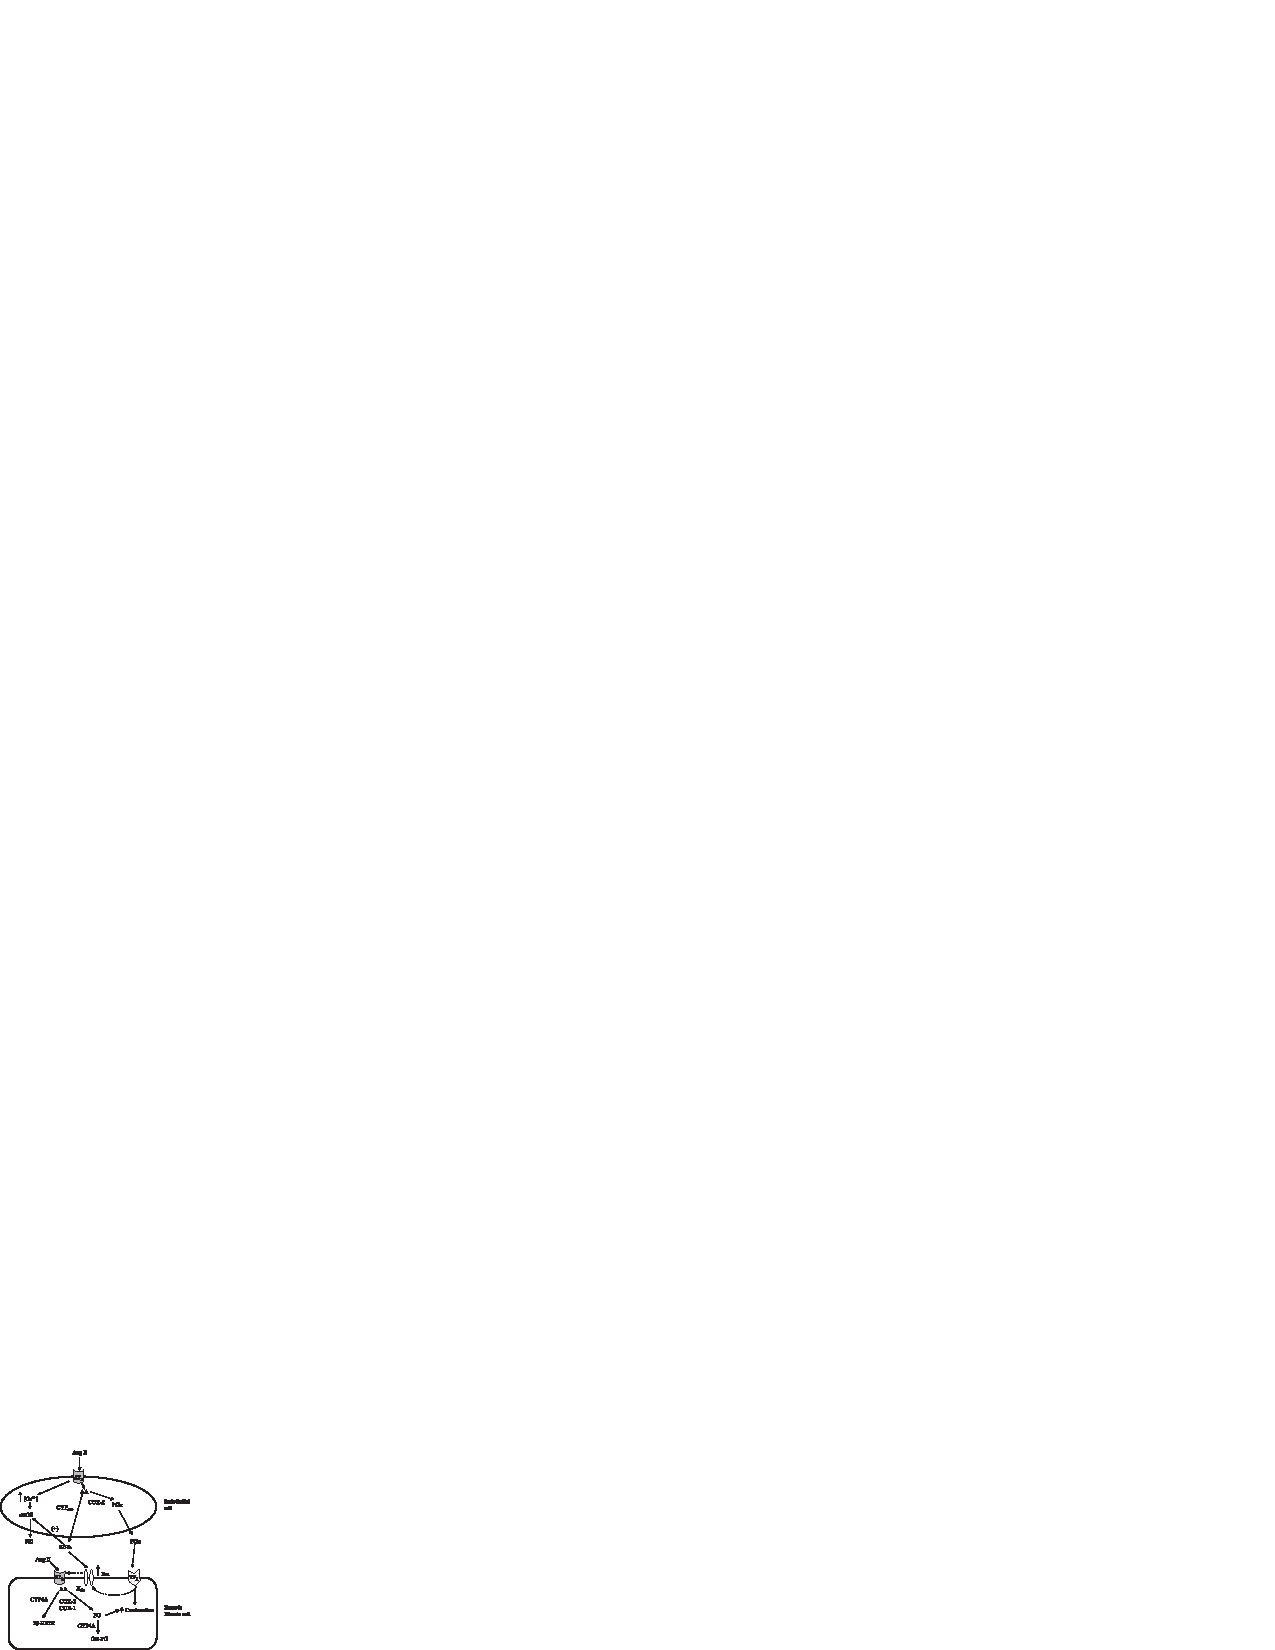
\includegraphics{fx1}\hspace*{5mm}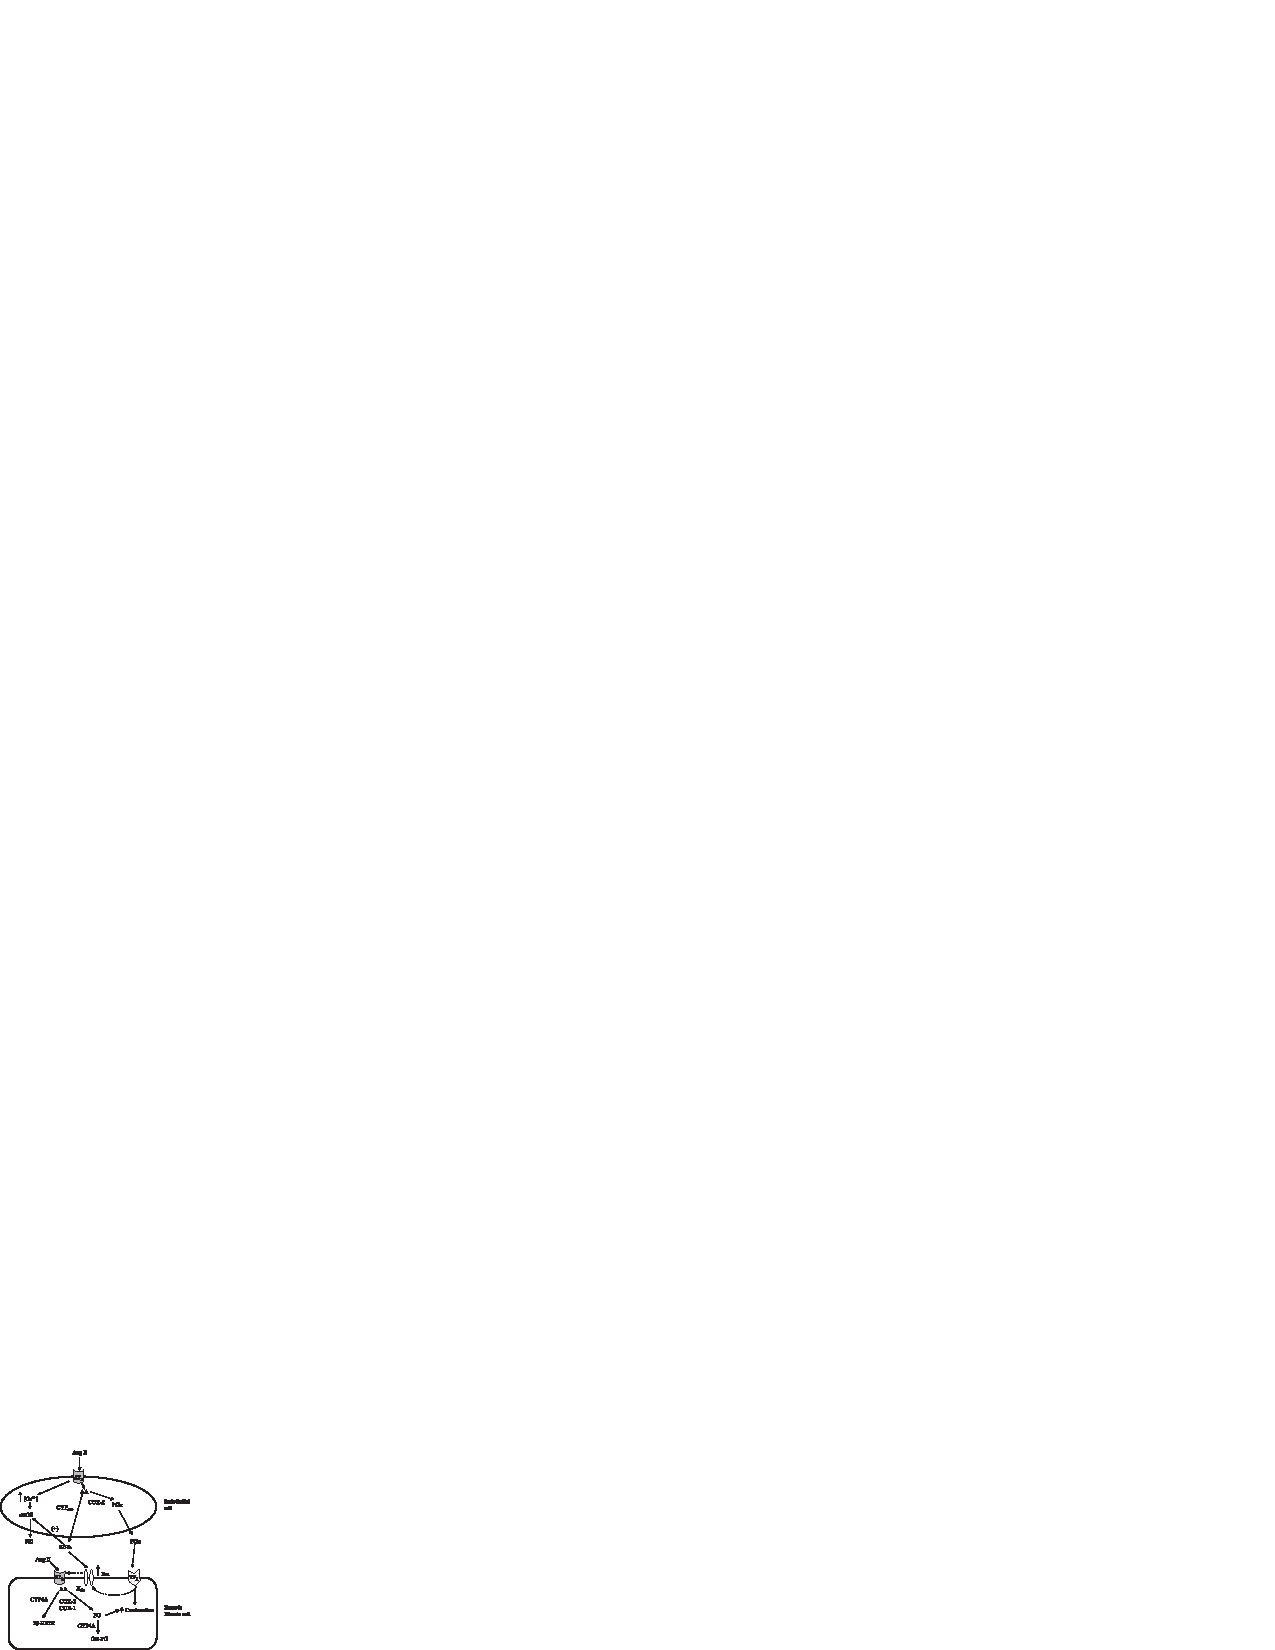
\includegraphics{fx1}}
%\centerline{
\includegraphics{gr1}}
%\caption{(a) first picture; (b) second picture.}
%\end{figure}

%The figure number and caption should be typed below the illustration in 8 pt and left justified [{{\bfseries\itshape Note:}} one-line captions of length less than column width (or full typesetting width or oblong) centered]. For more guidelines and information to help you submit high quality artwork please visit: http://www.elsevier.com/artworkinstructions\break Artwork has no text along the side of it in the main body of the text. However, if two images fit next to each other, these may be placed next to each other to save space. For example, see Fig.~1. 


%\section{Equations}
%Equations and formulae should be typed in Mathtype, and numbered consecutively with Arabic numerals in parentheses on the right hand side of the page (if referred to explicitly in the text). They should also be separated from the surrounding text by one space
%\begin{equation}
%\begin{array}{lcl}
%\displaystyle X_r &=& \displaystyle\dot{Q}^{''}_{rad}\left/\left(\dot{Q}^{''}_{rad} + \dot{Q}^{''}_{conv}\right)\right.\\[6pt]
%\displaystyle \rho &=& \displaystyle\frac{\vec{E}}{J_c(T={\rm const.})\cdot\left(P\cdot\left(\displaystyle\frac{\vec{E}}{E_c}\right)^m+(1-P)\right)}
%\end{array}
%\end{equation}


%\section{Online license transfer}
%All authors are required to complete the Procedia exclusive license transfer agreement before the article can be published, which they can do online. This transfer agreement enables Elsevier to protect the copyrighted material for the authors, but does not relinquish the authors' proprietary rights. The copyright transfer covers the exclusive rights to reproduce and distribute the article, including reprints, photographic reproductions, microfilm or any other reproductions of similar nature and translations. Authors are responsible for obtaining from the copyright holder, the permission to reproduce any figures for which copyright exists.








%\section*{Acknowledgements}

%Acknowledgements and Reference heading should be left justified, bold, with the first letter capitalized but have no numbers. Text below continues as normal.

%% The Appendices part is started with the command \appendix;
%% appendix sections are then done as normal sections
%% \appendix

%% \section{}
%% \label{}

%\appendix
%\section{An example appendix}
%Authors including an appendix section should do so before References section. Multiple appendices should all have headings in the style used above. They will automatically be ordered A, B, C etc.

%\subsection{Example of a sub-heading within an appendix}
%There is also the option to include a subheading within the Appendix if you wish.




%% Authors are advised to use a BibTeX database file for their reference list.
%% The provided style file elsarticle-num.bst formats references in the required Procedia style

%% For references without a BibTeX database:

% \begin{thebibliography}{}

%% \bibitem must have the following form:
%%   \bibitem{key}...
%%

%\bibitem[Clark et al.(1962)]{clark}Clark, T., Woodley, R., De Halas, D., 1962. Gas-Graphite Systems, in ``{\it Nuclear Graphite}''. 
%In: Nightingale, R. (Ed.). Academic Press, New York, pp. 387.

%\bibitem[Deal and Grove(2009) ]{Deal}Deal, B., Grove, A., 1965. General Relationship for the Thermal Oxidation of Silicon. Journal of Applied Physics 36, 37--70.

%\bibitem[Deep(2009)]{Deep}Deep-Burn Project: Annual Report for 2009, Idaho National Laboratory, Sept. 2009.

%\bibitem[Fachinger(2004)]{Fachinger2004}Fachinger, J., den Exter, M., Grambow, B., Holgerson, S., Landesmann, C., Titov, M., Podruhzina, T., 2004. ``Behavior of spent HTR fuel elements in aquatic phases of repository host rock formations,'' 2nd International Topical Meeting on High Temperature Reactor Technology. Beijing, China, paper \#B08. 

%\bibitem[Fachinger(2006)]{Fachinger2006}Fachinger, J., 2006. Behavior of HTR Fuel Elements in Aquatic Phases of Repository Host Rock Formations. Nuclear Engineering \& Design 236,     54.


 %\end{thebibliography}















%\clearpage

%%%% This page is for instructions only, once the article is finalize please omit the below text before creating the final PDF
%\normalMode

%\section*{Instructions to Authors for LaTeX template:}

%\section{ZIP mode for LaTeX template:}

%The zip package is created as per the guide lines present on the URL http://www.elsevier.com/author-schemas/ preparing-crc-journal-articles-with-latex for creating the LaTeX zip file of Procedia LaTeX template.  The zip generally contains the following files:
%\begin{Itemize}[]\leftskip-17.7pt\labelsep3.3pt
%\item ecrc.sty
%\item  elsarticle.cls
%\item elsdoc.pdf
%\item .bst file
%\item Manuscript templates for use with these bibliographic styles
%\item  Generic and journal specific logos, etc.
%\end{Itemize}

%The LaTeX package is the main LaTeX template. All LaTeX support files are required for LaTeX pdf generation from the LaTeX template package. 

%{\bf Reference style .bst file used for collaboration support:} In the LaTeX template packages of all Procedia titles a new ``.bst'' file is used which supports collaborations downloaded from the path http://www.elsevier.com/author-schemas/the-elsarticle-latex-document-class

%\section{Reference styles used in  Procedia master templates:}
%\let\footnotesize\normalsize
%\hspace*{-10pt}\begin{tabular*}{\hsize}{@{}ll@{}}
%{\bf Title}&{\bf Reference style} \\[6pt]
%AASPRO  & 2 Harvard\\
%AASRI Procedia  & 3 Vancouver Numbered\\
%APCBEE Procedia  & 3 Vancouver Numbered\\
%EGYPRO  & 3 Vancouver Numbered\\
%FINE    & 2 Harvard\\
%IERI Procedia  & 3 Vancouver Numbered\\
%MATPR  & 1a Numbered without article titles\\
%MSPRO  & 2 Harvard\\
%PHPRO  & 2 Harvard\\
%PIUTAM  & 3a Embellished Vancouver \\
%Procedia CIRP  & 3 Vancouver Numbered\\
%PROCHE  & 3a Embellished Vancouver \\
%PROCS  & 3a Embellished Vancouver \\
%PROENG  & 1 Numbered\\
%PROENV  & 3a Embellished Vancouver \\
%PROEPS  & 3a Embellished Vancouver \\
%PROFOO    & 3a Embellished Vancouver \\
%PROMFG  & 1a Numbered without article titles\\
%PROTCY  & 3 Vancouver Numbered\\
%PROVAC  & 3a Embellished Vancouver \\
%SBSPRO  & 5 APA\\
%SEPRO  & 3a Embellished Vancouver \\
%AQPRO & 2 Harvard\\
%UMKPRO & 5 APA\\
%TRPRO  & 2 Harvard\\
%\end{tabular*}









\end{document}

%%
%% End of file `procs-template.tex'.
